\documentclass{sig-alternate-05-2015}
\usepackage{paralist}
\usepackage{url}
\usepackage{hyperref}
\DeclareMathOperator{\lcm}{lcm}

\begin{document}
\setcopyright{acmcopyright}
\conferenceinfo{ISSAC 2017}{July 25--28, 2017, Kaiserslautern, Germany}

\newtheorem{alg}{Algorithm}
\newtheorem{definition}{Definition}
\newtheorem{lemma}{Lemma}
\newtheorem{theorem}{Theorem}
\newtheorem{Assertion}{Assertion}

\providecommand{\QQ}{\mathbb{Q}}
\providecommand{\ZZ}{\mathbb{Z}}
\providecommand{\NN}{\mathbb{N}}
\providecommand{\RR}{\mathbb{R}}
\providecommand{\CC}{\mathbb{C}}

\makeatletter
\def\Ddots{\mathinner{\mkern1mu\raise\p@
\vbox{\kern7\p@\hbox{.}}\mkern2mu
\raise4\p@\hbox{.}\mkern2mu\raise7\p@\hbox{.}\mkern1mu}}
\makeatother

\title{Nemo/Hecke: computer algebra and number theory packages for the Julia programming language}

\numberofauthors{4}
\author{
\alignauthor Claus Fieker\\
   \affaddr{TU Kaiserslautern}\\
   \affaddr{Fachbereich Mathematik, Postfach 3049,}\\
   \affaddr{67653 Kaiserslautern, Germany}\\
   \email{fieker@mathematik.uni-kl.de}
\alignauthor William Hart\\
   \affaddr{TU Kaiserslautern}\\
   \affaddr{Fachbereich Mathematik, Postfach 3049,}\\
   \affaddr{67653 Kaiserslautern, Germany}\\
   \email{goodwillhart@gmail.com}
\alignauthor Tommy Hofmann\\
   \affaddr{TU Kaiserslautern}\\
   \affaddr{Fachbereich Mathematik, Postfach 3049,}\\
   \affaddr{67653 Kaiserslautern, Germany}\\
   \email{thofmann@mathematik.uni-kl.de}
\and
\alignauthor Fredrik Johansson\\
   \affaddr{Inria Bordeaux \&}\\
   \affaddr{Institut de Math\'{e}matiques de Bordeaux} \\
   \affaddr{33400 Talence, France}\\
   \email{fredrik.johansson@gmail.com}
}

\maketitle

\begin{abstract}
We introduce two new packages, Nemo and Hecke, written in the Julia programming language
for computer algebra and number theory.
We demonstrate that high performance generic
algorithms can be implemented in Julia, without the need to resort to a low-level C
implementation. We also describe the various Julia wrappers of existing C/C++ libraries
such as Flint, Arb, Antic and Singular. We give examples of how to use Hecke and Nemo and discuss
some of the algorithms that we have implemented to provide high performance basic
arithmetic.
\end{abstract}


\section{Introduction}

Nemo is a computer algebra package for the Julia programming language. The eventual aim is
to provide highly performant commutative algebra, number theory, group theory and discrete
routines.

Nemo consists of two parts: wrappers of specialised C/C++
libraries (Flint \cite{flint}, Arb \cite{arb}, Antic \cite{antic} and Singular
\cite{singular}), and
implementations of generic algorithms and mathematical data
structures in the Julia language. So far the fully recursive constructions include
univariate polynomial rings, power series rings, residue rings (modulo principal ideals),
fraction fields, matrices and more recently multivariate polynomials with a sparse
distributed representation.

\subsection{The Julia programming language}

Julia \cite{julia} is a sophisticated, modern programming language which is designed
to be both performant and flexible.
The first public version of Julia appeared in 2012. 
Julia was written for technical computing with a
focus on numerics. However, it has found widespread use for many general purpose
applications, largely due to its innovative type system, dispatch mechanism, JIT
compilation and metaprogramming capabilities.
The benefits of Julia include:

\begin{itemize}
\item Familiar imperative syntax (like Python and Matlab), including support for operator overloading.
\item An interactive console, as well as Jupyter support (for web based notebooks).
\item Parametric types, multiple dispatch, and powerful metaprogramming facilities.
\item Just-In-Time compilation, supported by dynamic type inference.
\item Automatic memory management (garbage collection).
\item An efficient native C interface, and more recently an experimental C++ interface.
\item High performance collection types (dictionaries, iterators, arrays, etc.) and a powerful standard library.
\end{itemize}

Julia's JIT compilation allows fast performance for
generic algorithms. (Contrast: Python?... Alternative: C++ templates?)

One of the most important features from a mathematical point of view is Julia's parametric type system.
A type is parametric if it depends on another type. For example, in Julia, an array of integers has
type \texttt{Array\{Int, 1\}} (the 1 refers to the number of dimensions of the array).

We make heavy use of the parametric type system in Nemo and Hecke. For example, generic polynomials
over a ring $R$ have type \texttt{GenPoly\{T\}} where $T$ is the type of elements of the ring $R$.
Parametric types bear some resemblance to C++ template classes, but note that in Julia the type $T$ can
be constrained to belong to a specified class of types.

\section{Modelling domains in Julia}

Julia provides two levels of types that we make use of: abstract types and concrete types.
Concrete types are equivalent to the types that appear in languages such as Java, C or C++,
etc.

Abstract types can be thought of as collections of types. They are used when writing generic
functions that should work for any type in the given collection.

To write a generic function that accepts any type in a given collection of types, we first
create an abstract type. Then we create the individual concrete types that belong to that
abstract type. A generic function can then be constructed with a type parameter, T
say, similar to a template parameter in C++. The main difference is that we can specify
which abstract type our type parameter T must belong to.

In Julia, the symbol <: is used to specify that a given type belongs to a given abstract type.
For example the built-in Julia type Int64 for 64 bit machine integers belongs to the Julia
abstract type Integer.

Abstract types in Julia can form a hierarchy. For example, the Nemo.Field abstract type belongs
to the Nemo.Ring abstract type. An object representing a field in Nemo has type belonging to
Nemo.Field. But because we define the inclusion Nemo.Field <: Nemo.Ring, the type of such an
object also belongs to Nemo.Ring. This means that any generic function in Nemo which is designed
to work with ring objects will also work with field objects.

Julia always picks the most specific function that applies to a given type. This allows one to
implement a function at the most general level of a type hierarchy at which it applies. One can
also write a version of a given function for specific concrete types. For example, one may wish
to call a specific C implementation for a multiplication algorithm, say, when arguments with a
certain very specific given type are passed.

Another way that we make use of Julia's abstract type system in Nemo/Hecke is to distinguish
between the type of elements of fields, and the fields themselves, and similarly for all other
kinds of domains in Nemo. 

The diagram below shows the abstract type hierarchy in Nemo.

\begin{figure}[h]
\centering
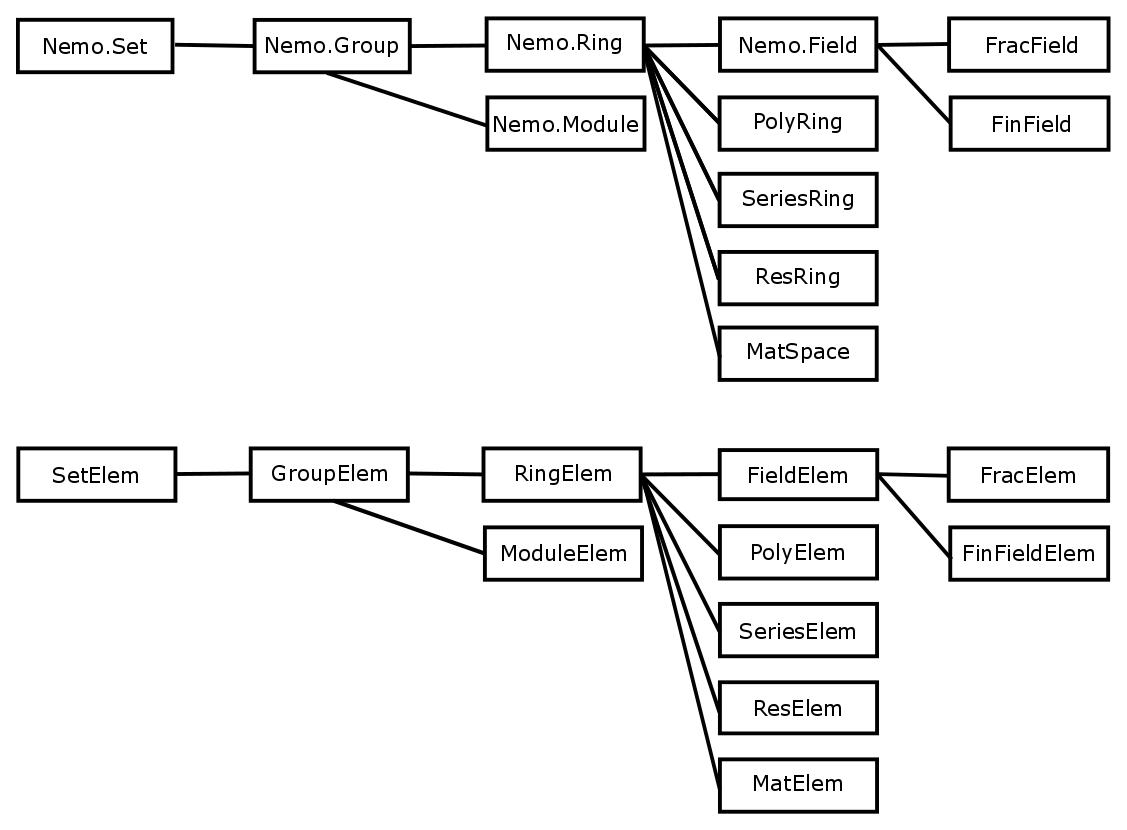
\includegraphics[scale=0.21]{types.png}
\caption{The Nemo abstract type hierarchy}
\end{figure}

Naively, one may expect that specific mathematical domains in Nemo/Hecke can be modeled as types
and their elements as objects of the given type. But there are various reasons why this is not a
good model.

As an example, consider the ring $R = \mathbb{Z}/n\mathbb{Z}$. If we were to model the ring $R$
as a type, then the type would need to contain information about the modulus $n$. This is not
possible in Julia if $n$ is an object, e.g. a multiprecision integer.

Putting such information in types is also not desirable. Julia dispatches on type, and each time
we call a generic function with different types, a new version of the function is compiled by the
JIT compiler. This would result in very poor performance if we were writing a multimodular
algorithm, say. In such an algorithm many rings $\mathbb{Z}/n\mathbb{Z}$ may be needed, and
recompilation would be triggered for each distinct $n$.

For this reason, the modulus $n$ needs to be attached to the elements of the ring, not to the type
associated with those elements.

The way we deal with this is to have special (singleton) objects, known as parent objects, that act
like types, but are in fact ordinary Julia objects. As ordinary objects, parents can contain
arbitrary information, such as the modulus in $\mathbb{Z}/n\mathbb{Z}$. Each element in the ring
$\mathbb{Z}/n\mathbb{Z}$ then contains a pointer to the relevant parent object.

This model of mathematical parent objects is taken from SageMath \cite{sage} which in turn followed
the Magma \cite{magma} computer algebra system.

Julia allows ordinary objects to be made callable. We make use of the facility to write coercions
and constructors for elements of mathematical domains in Nemo/Hecke. For example, the following
code constructs $a = 3 \pmod{7}$.

\begin{verbatim}
R = ResidueRing(ZZ, 7)
a = R(3)
\end{verbatim}

We also make use of the parent object system to encode information such as context objects needed
by C libraries. As Julia objects can have precisely the same bit representation as native C objects,
parent objects can be passed directly to C functions. Additional fields in these objects can safely
appended if it is desirable to retain more information at the Julia level than the C/C++ level. 

\section{Nemo: basic arithmetic in Julia}

Julia was designed with high performance numerical algorithms in mind, and can be used to
implement numerical algorithms involving floating point numbers at essentially the same
speed as a low-level C or Fortran algorithm. 

It is remarkable that the performance of Julia is so close to C in the optimum case that
it is possible to implement fast basic arithmetic in Julia itself. We view the main
advantage of Julia as the ability to implement fast generic algorithms, for which a specific
implementation does not exist in C. It is also quite convenient to prototype low level
algorithms in Julia and then port this to low level, hand optimised C with manual memory
management at a later stage.

Of course, many algebraic applications depend on fast assembly optimised bignum arithmetic
which Julia is unlikely to be able to compete with. In fact, Julia itself wraps the GMP
\cite{gmp} and MPFR \cite{mpfr} libraries for its own multiprecision arithmetic.

In this section, we present a few code examples which also double as
benchmark problems.
Additional benchmarks are available
at \url{http://nemocas.org/benchmarks.html}.

\subsection{Multivariate polynomials}

We first consider arithmetic in $\mathbb{Z}[x_1,\ldots,x_k]$.
The Fateman benchmark consists of computing
$f \cdot (f+1)$ where $f = (1 + x + y + z + t)^n$,
usually with $n = 30$. In Nemo, this is expressed by the following code:

\begin{verbatim}
R,x,y,z,t = PolynomialRing(ZZ, ["x","y","z","t"])
f = (1+x+y+z+t)^30
f*(f+1)
\end{verbatim}

Table~\ref{tab:fateman} shows timing results compared to
SageMath~7.4, Magma~V2.22-5 and Giac-1.2.2
on a 2.2~GHz AMD Opteron 6174.
We used sparse multivariate polynomials in all
cases (this benchmark could also be performed
using nested univariate arithmetic, i.e. in $\mathbb{Z}[x][y][z][t]$).

Nemo (generic) is our implementation of Johnson's sparse
multiplication algorithm for generic coefficients in Julia.
This implementation is not used by default over $\mathbb{Z}$, but we
have included it here to give a comparison between
Julia and C.
Flint (no asm) is our implementation of essentially
the same algorithm in C specifically for the coefficient ring $\mathbb{Z}$,
and Flint (asm) is the same with additional
assembly optimisations for the coefficient arithmetic.

Finally, Flint (array) and Giac implement an algorithm designed
for dense polynomials, which consists of accumulating all terms
into a big array covering all possible exponents.
(These polynomials are too sparse on a rectangular support
for Kronecker segmentation to be effective, which otherwise
would be the preferred way to multiply dense polynomials.)

Table~\ref{tab:pearce} shows timing results on the Pearce
benchmark, which consists of computing $f \cdot g$ where
$f = (1 + x + y + 2z^2 + 3t^3 + 5u^5)^n$,
$g = (1 + u + t + 2z^2 + 3y^3 + 5x^5)^n$.
This problem is too sparse to use the big array method,
so only the Johnson algorithm is used.
As before, we compare the generic Julia version
with Flint (with and without assembly optimisations).
Here Giac likewise uses a fully sparse algorithm.

\begin{table}
\center
\caption{Time (s) on the Fateman benchmark.}
\begin{small}
\setlength{\tabcolsep}{2.5pt}
\renewcommand{\arraystretch}{1.2}
\begin{tabular}{c c c c c c c c} \hline
$n$ & SageMath & Magma & Nemo & Flint & Flint & Flint & Giac \\ 
    &          &       & (generic) & (no asm) & (asm) & (array) & \\ \hline
     5  &  0.008 & $\sim$0.01   & 0.004      &        0.002    &        0.002       &      0.0003    &    0.0002 \\
    10  &  0.53  &   0.12  &   0.11     &         0.04    &         0.02       &         0.005   &      0.006 \\
    15  &   10   &    1.9  &      1.6   &         0.53    &          0.30      &           0.08   &         0.11 \\
    20  &   76   &    16   &    14.3    &          6.3    &            2.8     &            0.53   &         0.62 \\
    25  &  426   &   98    &      82    &          39     &         17.4        &           2.5     &         2.8 \\
    30  & 1814   & 439     &  362       &         168     &            82        &            11     &          14 \\
\end{tabular}
\label{tab:fateman}
\end{small}
\end{table}

We emphasise again that Nemo defaults to using Flint instead of the generic
Julia code for $\mathbb{Z}[x_1,\ldots,x_k]$.
Flint in turn will use the (array) method by default
given sufficiently dense input (e.g.\ on the Fateman polynomials)
and the assembly optimised Johnson algorithm otherwise (e.g.\ on the Pearce polynomials).

It is somewhat remarkable that the generic Julia implementation
of Johnson's algorithm comes
within a factor two of our C version in Flint (without asm),
and even runs slightly faster than the C code in Magma.
Of course, the coefficient ring $\mathbb{Z}$ is exceptionally important
so even small speedups matter,
and arithmetic in $\mathbb{Z}$ is cheap
(and susceptible to precisely the type of low level optimisations
that are convenient to do in C), which is why we go through
the trouble to write a dedicated implementation of $\mathbb{Z}[x_1,\ldots,x_k]$ in Flint.
Over more exotic coefficient domains, the relative
overhead of the generic Julia code will be even less significant,
making specialied C implementations less useful.

\begin{table}
\center
\caption{Time (s) on the Pearce benchmark.}
\begin{small}
\setlength{\tabcolsep}{2.5pt}
\renewcommand{\arraystretch}{1.2}
\begin{tabular}{c c c c c c c} \hline
$n$ & SageMath & Magma & Nemo & Flint & Flint & Giac \\ 
    &          &       & (generic) & (no asm) & (asm) & \\ \hline
     4  &   0.01 & $\sim$0.01  &   0.008          & 0.003         &   0.002             &                     0.004 \\
     6  &   0.20  &   0.08   &     0.07        &     0.03       &       0.03         &                           0.03 \\
     8  &   2.0  &     0.68   &     0.56       &      0.16      &        0.15        &                            0.28 \\
    10  &   11   &     3.0    &       2.2      &       0.77     &         0.71       &                             1.45 \\
    12  &   57   &    11.3    &      8.8       &        3.7     &           3.2      &                                4.8 \\
    14  &  214   &   36.8     &   32.3         &       16       &         12         &                               14 \\
    16  &  785   &   94.0     &   85.5         &       44       &         32         &                               39 \\
\end{tabular}
\label{tab:pearce}
\end{small}
\end{table}

\subsection{Generic resultant}

The following example computes a resultant
in the ring $((\operatorname{GF}(17^{11})[y])/(y^3 + 3xy + 1))[z]$,
demonstrating generic recursive rings and polynomial
arithmetic. Flint is used for univariate polynomials over a finite field.

\begin{verbatim}
R, x = FiniteField(7, 11, "x")
S, y = PolynomialRing(R, "y")
T = ResidueRing(S, y^3 + 3x*y + 1)
U, z = PolynomialRing(T, "z")

f = (3y^2+y+x)*z^2 + ((x+2)*y^2+x+1)*z + 4x*y + 3
g = (7y^2-y+2x+7)*z^2 + (3y^2+4x+1)*z + (2x+1)*y + 1

s = f^12
t = (s + g)^12
resultant(s, t)
\end{verbatim}

This example takes 179907~s in SageMath~6.8, 82 s in Magma V2.21-4
and 0.2 s in Nemo-0.4.

\subsection{Generic linear algebra}

We compute the determinant of a random $80\times80$ matrix
with entries in a cubic number field.
This benchmark is designed to test generic linear algebra over a field
where there is coefficient blowup. The number field arithmetic is
provided by Antic.

\begin{verbatim}
QQx, x = PolynomialRing(QQ, "x")
K, a = NumberField(x^3 + 3*x + 1, "a")
M = MatrixSpace(K, 80, 80)()

for i in 1:80
 for j in 1:80
   for k in 0:2
     M[i, j] = M[i, j] + a^k * (rand(-100:100))
   end
 end
end

det(M)
\end{verbatim}

This takes 5893~s in SageMath~6.8, 21.9~s in Pari/GP~2.7.4 \cite{pari}, 5.3~s in Magma V2.21-4,
and 2.4~s in Nemo-0.4.

\section{Generic algorithms in Nemo}

Many high level algorithms in number theory and computer algebra rely on
the efficient implementation of fundamental algorithms.

\subsection{In-place operations}

A consistent way to improve performance is to modify
elements in-place, especially when making incremental updates
to large, highly nested objects.
In-place operations are used pervasively in Flint (and one level below, in GMP/MPIR).
Nemo objects are ostensibly immutable, but local mutation is
acceptable while an object is being created,
and Nemo provides special methods for this purpose.
For recursively constructed objects, the in-place methods work
recursively down to and including the ground level C objects.
Thus, instead of writing
\begin{verbatim}
s += a * b
\end{verbatim}
which creates an object for \texttt{a * b}
and then replaces \texttt{s} with yet another new object, we may
create a scratch variable \texttt{t} with the same type as \texttt{a}, \texttt{b} and \texttt{s} and use
\begin{verbatim}
mul!(t, a, b)
addeq!(s, t)
\end{verbatim}
which creates no new objects and avoids making a copy of the data in \texttt{s}
that is not being modified.
Naturally, the idea is to limit this less readable construct to
critical inner loops of operations such as polynomial
and matrix multiplication.
%Using this in-place update in the main loop of univariate polynomial
%multiplication saves a whole factor 6.7 on the Fateman benchmark
%$f \cdot (f+1)$ where
%$f = (1 + x + y + z + t)^{30}$, evaluated over the nested univariate
%ring $\mathbb{Z}[x][y][z][t]$. This is an extreme example, and
%the typical gain is more modest.

\subsection{Polynomial algorithms}

For dense univariate polynomials over a commutative ring we implement classical
polynomial multiplication. However, when the base ring is itself a polynomial ring,
we have available an implementation of Kronecker segmentation, to reduce the
multivariate multiplication to the univariate case.

For use in the subresultant GCD algorithm, we implement generic, polynomial
pseudoremainder. 

The generic polynomial resultant code computes the resultant using subresultant
pseudoremainder sequences. This code can even be called for polynomials over a
ring with zero divisors, so long as impossible inverses are caught. The exception
can be caught using a try/catch block in Julia and a fallback method called, e.g.
the resultant can be computed using Sylvester matrices. This allows an algorithm
with quadratic complexity to be called generically, with an algorithm of cubic
complexity only called as backup in case of failure.

For generic power series, Nemo implements both relative and absolute
representations. In the relative case, the valuation is stored separately so that
the internal representation begins with the first nonzero coefficient (for nonzero
power series). This greatly speeds up working with power series that have large
valuation.

For powering we usually make use of the standard square-and-add approach. However
when a polynomial with few terms is raised to a high power, we make use of the
multinomial powering algorithm.

Nemo also provides a module for generic multivariate polynomials in sparse distributed
format. We made use of variants of the sparse algorithms described by Monagan and
Pearce for heap-based multiplication \cite{heapmul}, exact division and division with
remainder \cite{heapdiv} and powering \cite{heappow}.

In the case of pseudodivision for sparse, multivariate polynomials, we extract one
of the variables and then implement a heap-based, univariate pseudoremainder
algorithm inspired by an unpublished manuscript of Monagan and Pearce.

We make use of this pseudoremainder implementation to implement the subresultant
GCD algorithm. To speed this up, we make use of a number of tricks employed by the
Giac/XCAS system \cite{giac}, as taught to us by Bernard Parisse. The most important
of these is cheap removal of the content that accumulates during the subresultant
algorithm by analysing the input polynomials to see what form the leading coefficient
of the GCD can take.

We also use heuristics to determine which permutation of the variables will lead to
the GCD being computed in the fastest time. This heuristic favours the variable with
the lowest degree as the main variable for the computation, with the other variables 
following in increasing order of degree thereafter. But our heuristic heavily favours
variables in which the polynomial is monic.

\subsection{Matrix algorithms}

Here we describe some of the linear algebra improvements and algorithms for matrices
over generic commutative rings that we have implemented in Nemo.

For computing the determinant over a generic commutative ring, we implemented a generic
algorithm making use of Clow sequences \cite{clow} which uses only $O(n^4)$ ring operations
in the dimension $n$ of the matrix. However, two other approaches seem to always outperform
it. The first approach makes use of a generic fraction free LU decomposition. This algorithm
may fail if an impossible inverse is encountered. However, as a fallback, we make use of a
division free determinant algorithm. This computes the characteristic polynomial and then
extracts the determinant from that.

For determinants of matrices over polynomial rings, we use an interpolation approach.

We implemented an algorithm for computing the characteristic polynomial due to
Danilevsky (see below) and an algorithm that is based on computing the Hessenberg
form. We also make use of a generic implementation of the algorithm of Berkowitz which
is division free. 

As is well known, fraction free algorithms often improve the performance of matrix
algorithms over an integral domain. For example, fraction free Gaussian elimination
for LU decomposition, inverse, determinant and reduced row echelon form
are well-known.

In addition we have been able to use this strategy in the computation
of the characteristic polynomial. We have adapted the well-known 1937 method
of Danilevsky for computing the characteristic polynomial into a fraction-free
version.

Danilevsky's method works by applying similarity transforms to reduce the
matrix to Frobenius form. Normally such computations are computed over a
field, however each of the outer iterations in the algorithm introduce only
a single denominator. Scaling by this denominator allows us to avoid
fractions.

Of course this then introduces the problem that the entries become larger
as the algorithm proceeds because of the scaling. However, conveniently
it is possible to prove that the introduced scaling factor can be removed 
one step later in the algorithm. This is an exact division and doesn't
lead to denominators.

Removing such a factor has to be done in a way that respects the
similarity transforms. We achieve this by making two passes over the matrix
to remove the common factor.

FIXME: talk about matrix algorithms over rings.

\subsubsection{Minimal polynomial}

Next we describe an algorithm we have implemented for efficient
computation of minimal polynomial of an $n\times n$ integer matrix $M$.

A standard approach to this problem is known as ``spinning''. 
We first describe this idea for matrices over a field~$K$.

The main idea is to think of $M$ as a linear operator on an $n$-dimensional
$K$-vector space $V$ and to write $V$ as a sum of invariant subspaces, 
$V = W_1 + W_2 + \cdots + W_k$. If the restriction of $M$ to $W_i$ has
minimal polynomial $f_i$ then the minimal polynomial of $M$ is
$\lcm(f_1, f_2, \ldots, f_k)$.

To generate such subspaces we construct so-called Krylov sequences. Given
a vector $v \in V$ the Krylov subspace associated to $v$ is the linear
subspace spanned by $\{v, Mv, M^2v, \ldots\}$.

One way to get the minimal polynomial of $M$ heuristically is to choose
random vectors $v$, compute the associated Krylov subspaces and take their
minimal polynomials $f_i$. When the least common multiple of such minimal
polynomials stabilises, we have with high probability computed the minimal
polynomial of $M$.

However, a proof of termination can also be given as follows. Suppose that
we have vectors $v_1, v_2, \ldots, v_k$ such that their associated Krylov
subspaces $W_1, W_2, \ldots, W_n$ are pairwise distinct and that their
sum is $V$. Then the least common multiple of their minimal polynomials is
the minimal polynomial of $M$.

Instead of choosing random vectors $v_i$, our algorithm starts with
$v_1 = e_1 = (1, 0, 0, \ldots, 0)$ and at each step chooses $v_i$ to be
the first standard basis vector $e_j$ that is linearly independent of the
Krylov subspaces $W_1, W_2, \ldots, W_{i-1}$ computed so far.

We keep track of which standard basis vectors are independent by
incrementally reducing a matrix $B$ whose rows consist of all the
linearly independent vectors from the Krylov sequences computed so
far.

Any column without a pivot in this reduced matrix $B$ corresponds to a
standard basis vector which is independent of the Krylov subspaces
computed so far.

Once the rank of this incrementally reduced matrix $B$ reaches $n$, the sum
of the Krylov subspaces we have computed is $V$ and we are done.

In order to compute the minimal polynomial of a matrix $M$ over $\mathbb{Z}$,
we make use of a multimodular approach, reducing the matrix $M$ modulo many
small primes $p$ and applying the method described above. We then combine
the minimal polynomials modulo the various primes $p$ using Chinese
remaindering.

The only difficulty is knowing when to stop. Heuristically this happens
when the Chinese remaindering stabilises. Whilst bounds on the number of
primes required do exist, e.g. based on Ovals of Cassini, the bounds are
typically extremely pessimistic. We prefer stop as soon as the Chinese
remaindering stabilises, but we need a proof of termination. 

It is unfortunately way too expensive to simply evaluate the minimal
polynomial $f$ at the matrix $M$ to see if it is zero, since this requires
taking powers of the matrix $M$, which requires $O(n^4)$ operations over
$\mathbb{Z}$ in total, in the worst case.

In order to give a proof of termination, we instead allow a small amount of
information to leak from the modulo~$p$ minimal polynomial computations.
Namely, we wish to know which standard basis vectors were used as
generators of the Krylov subspaces modulo~$p$. We observe that these are
almost always the same standard basis vectors for all primes~$p$ due to the
deterministic way we choose these as the first standard basis vector not
in the sum of the Krylov subspaces computed so far. 

Combining all the generators of the Krylov subspaces for all the primes~$p$
then gives us a small set of generators $v_i$ for the Krylov subspaces over
$\mathbb{Z}$ (not necessarily a minimal set).

Suppose that  $f$ is a purported minimal polynomial that is believed
heuristically to be correct, since the Chinese remaindering has stabilised.
On average, it is relatively cheap to compute $f(M)v_i$ for each such
vector $v_i$. If $f(M)v_i = 0$ for each of the vectors $v_i$ then $f$ is
in fact the minimal polynomial.

In the worst case this algorithm still requires $O(n^4)$ operations, but
this is far from the average case, even when the minimal polynomial is not
the characteristic polynomial.

Of course we know that the associated Krylov subspaces $W_i$ sum to $V$
because they do so modulo $p$.

We have been informed by personal communication that the algorithm used by
Magma \cite{magma} also uses spinning, however it uses a $p$-adic
approach over $\mathbb{Z}$. Unfortunately we have not been able to find a
publication outlining their method.

In practice our multimodular algorithm seems to slightly outperform Magma on the
examples we have tried, including matrices with minimal polynomial smaller 
than the characteristic polynomial.

A generic version of this algorithm is implemented in Julia code in Nemo, and
an efficient version over $\mathbb{Z}$ using the Chinese remaindering trick
is implemented in Flint and made available in Nemo.

\section{Hecke: algebraic number theory in Julia}

Hecke is a tool for algebraic number theory, written in the Julia programming language.
Initially developed during the DFG priority project SPP 1489, Hecke includes the following functionality:
\begin{itemize}
\item
  element and ideal arithmetic in orders of number fields,
\item
  class group and unit group computation,
\item
  verified computations with embeddings and
\item
  verified residue computation of Dedekind zeta functions.
\end{itemize}

Hecke is written purely in Julia and uses Nemo in two essential ways. On the one hand, it makes heavy use of Flint, Arb and Antic through the Julia interface provided by Nemo.
On the other hand, it applies the generic constructions and algorithms provided by Nemo to its own types. This allows for example to work efficiently with polynomials or matrices over rings of integers without the necessity to define special types for these objects.

While for most of the computational challenges we relied on well known techniques as described in \cite{Cohen1993, Pohst1997, Belabas2004} (with a few modifications), we use new strategies for ideal arithmetic as well as for computations with approximations.

\subsection{Fast ideal arithmetic in rings of integers}

A classical result is that in Dedekind domains, like the ring of integers of a number field, any
ideal can be generated using only two elements, one of which can even be chosen
at random in the ideal. From the very onset of algorithmic theory this was
tempting as it reduces the storage requirement to two elements in comparison to the many elements necessary to
store a $\ZZ$-basis. However, the key problem was always the lack of
efficient algorithms for working with the generators. We remark that one
operation was always efficient using two generators: powering of ideals.

A refinement of this idea, due to Pohst and Zassenhaus \cite[p. 400]{Pohst1997}, is that
of a \textit{normal} presentation. Here a finite set $S$ of prime numbers
is fixed, typically containing at least all prime divisors of the norm of the ideal. Then,
based on this set, the two generators are chosen: The first as an integer
having only divisors in $S$---but typically with too high multiplicities.
The second generator then has the correct multiplicity at all prime ideals
over primes in $S$---but is allowed to have other divisors as well.
For the remainder of this section, let $K/\QQ$ be a number field of
degree $n$ and $\mathcal O_K$ be its ring of integers.

\begin{definition}
Let $S$ be a finite set of prime numbers and $A$ a nonzero ideal such that
all primes $p$ dividing the norm $N(A) = |\mathcal O_K/A|$ are in $S$.
A tuple $(a, \alpha)$ is a $S$-normal presentation for $A$ if and only if
\begin{itemize}
\item we have $a\in A\cap \mathbb Z$, $\alpha\in A$,
\item for all prime ideals $Q$ lying over $p\not\in S$ we have $v_Q(a)= v_Q(A) = 0$
  for the exponential valuation $v_Q$ associated to $Q$,
\item for all prime ideals $Q$ over $p\in S$ we have $v_Q(\alpha) = v_Q(A)$.
\end{itemize}
\end{definition}

A direct application of the Chinese remainder theorem shows the existence of such normal presentations.
The algorithmic importance comes from the following result.

\begin{theorem}
Let $A = \langle a, \alpha \rangle$ be an ideal in $S$-normal presentation. Then the following hold:
\begin{enumerate}
\item We have $N(A) = \gcd(a^n, N(\alpha))$
\item If $B = \langle b, \beta\rangle$ is a second ideal in $S$-normal
presentation for the same set $S$, then
$AB = \langle ab, \alpha\beta\rangle$ is also a $S$-normal presentation.
\item Let $\gamma = 1/\alpha$, $\langle g\rangle = \alpha \mathcal O_K \cap \ZZ$,
 $g = g_1g_2$ with coprime $g_1$, $g_2$ and $g_2$ only divisible be primes not in $S$. Then $A^{-1} = \langle 1, g_2\gamma\rangle$ is a $S$-normal presentation.
\item If $p$ is a prime number and $P= \langle p, \theta\rangle$ a prime ideal over $p$
in $\{p\}$-normal presentation, then the $\{p\}$-normal presentation
of $P^{-1} = \langle 1, \gamma\rangle$ yields a valuation element, that is,
$v_P(\beta) = \max\{ k \mid \gamma^k\beta\in \mathcal O_K\}$ for all $\beta \in \mathcal O_K$.
\end{enumerate}
\end{theorem}

It should be noted that (almost all) prime ideal are naturally computed
in $\{p\}$-normal presentation. The key problem in using the theorem for
multiplication lies in the fact that both ideals need to be giving by a $S$-normal presentation for
the same set $S$, which traditionally is achieved by recomputing
a suitable presentation from scratch, taking random candidates for the
second generator until it works. Based on the following lemma, have developed a new algorithm that does it at the cost 
of a few integer operations only.

\begin{lemma}
Let $S$ be a finite set of prime numbers and $A=\langle a, \alpha\rangle$ an ideal in
$S$-normal presentation. Let $T$ be a second set of primes and set
$s = \prod_{x\in S} x$ as well as $t = \prod_{x\in T\setminus S} x$. If $1 = \gcd(as, t) = uas + vt$,
then $\langle a, \beta \rangle$ is a $S\cup T$-normal presentation, where $\beta = vt\alpha + uas$.
\end{lemma}

\begin{proof}
By definition, $a$ has only prime divisors in $S$, so $as$ and $t$ are coprime.
Also, $a$ is a possible first generator for the $S\cup T$-normal presentation.
Let $P$ be a prime ideal over a prime $p\in S$, then
$v_P(\beta) = v_P(\alpha)= v_P(A)$ since $v_P(A) <v_P(s)+v_P(a)$ due to $v_P(s)\ge 1$ and $v_P(a) \ge v_P(A)$ by definition.
For $P$ coming from $T\setminus S$, we have $v_P(\beta) = 0$ since $v_P(t)\ge 1$ and $v_P(uas) = 0$ as well.
\end{proof}

Using this lemma on both input ideals, we can get compatible $S$-normal 
presentations at the cost of two $\gcd$ computations, a few pure integer multiplications and two products of integers with algebraic numbers. The final ideal
multiplication is then a single integer product and a single product of
algebraic numbers. Thus the asymptotic cost is that of a single multiplication of two algebraic numbers.
In contrast, all previous algorithms required some linear algebra step.

Finally, we improve on the computation of a $S$-normal presentation.

\begin{lemma}
If $0\ne\alpha\in \mathcal O_K$, then $\langle\alpha\rangle\cap \mathbb Z = \langle d\rangle$ where $d>0$ is minimal such that $d/\alpha\in \mathcal O_K$.
\end{lemma}

\begin{theorem}[\cite{Pohst1997}]
Let $A$ be a nonzero ideal. Then
$(a, \alpha)$ is an $\{p \text{ prime} \mid p \text{ divides }a\}$-normal presentation for $A$ if and only if
for $d = \min \alpha\mathcal O_K \cap \NN$ we have
\[ \gcd(a, \frac{d}{\gcd(a, d)}) = 1.\]
\end{theorem}

Together with the above lemma, this allows for the rapid computation of a
normal presentation: Choose $\alpha\in A$ at random until a normal presentation
is obtained. It can be shown that, unless $a$ involves many ideals of small
norm, this is very efficient.

To illustrate the speed of our algorithm, we created a list of ideals of bounded norm (here: 400) and
took random products of 100 ideals in the field
defined by the polynomial $X^n + 2$ for $n=16, 32, 64, 128$.
The results are presented in the following table.
Times are given in seconds. A dash indicates that the computation took  more than 20 seconds.
\begin{center}
\begin{tabular}{c||c|c|c|c}
$n$ & 16 & 32 & 64 & 128 \\\hline
Magma & 14 & -& - & -        \\
Pari & 0.05 & 0.18 & 0.96 & 5.4 \\
Hecke & 0.02 & 0.04 & 0.06 & 0.08
\end{tabular}
\end{center}

%%
%% Pari:
%% #
%% n = nfinit(x^128+2);
%% p = 2
%% a = List([])
%% for(i=1, 100, j = idealprimedec(n, p); for(l=1, length(j), if(idealnorm(n, j[l]) < 400, listput(a, j[l]))); p = nextprime(p+1))
%% 
%% z = a[1]
%% for(i=1, 100, z = idealmul(n, z, a[1+random(length(a))]))
%%
%% Magma:
%% K := NumberField(x^16+2);
%% M := MaximalOrder(K);
%% F := FactorBasis(M, 400);
%% z := F[1];
%% time for i:= 1 to 10 do z *:= Random(F); end for;
%%
%% Hecke:
%% Qx, x = QQ["x"];
%% K, a  = NumberField(x^64+2);
%% O = maximal_order(K);
%% const B = Hecke.NfFactorBase(), 400; complete = false, degree_limit = 0)
%% z = B.ideals[1]
%% @time for i=1:100 z *= rand(B.ideals); end;

\subsection{The use of interval arithmetic}

While algebraic number fields and their elements have by definition a very algebraic character, very often one is forced to study these discrete objects in a real or complex setting, e.g. when using embeddings into an algebraically closed field or Dedekind zeta functions.
The necessity to do this can be twofold. On the one hand it could be an intrinsic property of the problem, and on the other hand it could be the fastest (known) way to solve a particular problem.
But no matter what the reason is, leaving the realm of discrete objects usually comes at the prize of working with approximations and all kinds of related complications.
We give a few examples of such instances and show, how the ball arithmetic provided by Arb is employed in Hecke to make working with these real and complex objects like a breeze.

\subsubsection{Computing conjugates}\label{subsub:conj}

Let $K = \QQ[X]/(f)$ be an algebraic number field, where $f \in \QQ[X]$ is an irreducible polynomial of degree $d$.
We represent the elements of $K$ as polynomials of degree less than $d$.
Denoting by $\alpha_1,\dotsc,\alpha_d \in \CC$ the roots of $f$ in $\CC$, the distinct embeddings $K \to \CC$ are given by $\sigma_i \colon K \to \CC, \bar X \mapsto \alpha_i$. For an element $\alpha$ of $K$ the complex numbers $\sigma_i(\alpha)$, $1 \leq i \leq d$ are called the conjugates of $\alpha$.
Since for $\alpha \in K \setminus \QQ$ the conjugates are irrational, it is clear that we cannot do exact computations with these objects but have to rely on approximation techniques.
In Hecke this is done using ball arithmetic. Let $\alpha = \sum a_j X^j$ be an element of $K$. 
Assume that we want to find $\hat \sigma_i(\alpha) \in \RR$ with $\lvert \sigma_i(\alpha) - \hat \sigma_i(\alpha) \rvert \leq 2^{-p}$ for some precision $p \in \ZZ_{\geq 1}$.
Using Arb's polynomial root finding functionality and some initial precision $p' \geq p$ we can find balls $B_{p'}^{(i)} \subseteq \RR$ such that $\alpha_i \in B_{p'}^{(i)}$ and $\operatorname{diam}(B_{p'}^{(i)}) \leq 2^{-p'}$.
Ball arithmetic then yields balls $B_\alpha^{(i)} \subseteq \RR$ with
\[ \sigma_i(\alpha) = \sum_{1 \leq j \leq d} a_j \alpha_i^j \in \sum_{1 \leq j \leq d} a_j (B_{p'}^{(i)})^j\subseteq B_\alpha^{(i)}. \]
Finally we check whether $\operatorname{diam}(B_\alpha^{(i)}) \leq 2^{-p}$. If this is not the case, we increase the working precision $p'$ and repeat the steps.
When finished, the midpoints of the balls $B_\alpha^{(i)}$ are approximations $\hat \sigma_i(\alpha)$ with the desired property.
The following code shows how this can be implemented in Hecke.

\begin{verbatim}
QQx, x = PolynomialRing(QQ, "x")
K, a = NumberField(x^3 + 3*x + 1, "a")
alpha = a^2 + a + 1
p = 128
p' = p

while true
  CCy, y = PolynomialRing(AcbField(p'), "y")
  g = CCy(x^3 + 3*x + 1)
  rts = roots(g)
  z = map(x^3 + x + 1, rts)
  if all([ radiuslttwopower(u, -p) for u in z])
    break
  else
    p' = 2*p'
  end
end
\end{verbatim}

Performing the same task using only floating point arithmetic requires a priori error analysis to obtain the precision necessary for a correct result.
Since through the use of ball arithmetic the problem of keeping track of errors is delegated to Arb, this allows for quick development of algorithms working with conjugates, which at the same time yield guaranteed results.

\subsubsection{Torsion units}

For an algebraic number field $K$ of degree $d$, the set $\{ \alpha \in K^\times \mid \exists n \in \ZZ_{\geq 1} \colon \alpha^n = 1 \}$ of torsion units is a finite cyclic subgroup of $K^\times$, which plays an important role
when investigating the unit group of the ring of integers of $K$.
In particular for a given $\alpha \in K^\times$ it is important to quickly decide whether it is a torsion unit.
A list of possible integers $n$ with $\alpha^n = 1$ can be obtained as follows:
If $\alpha$ is a torsion unit, then $\alpha$ is a primitive $k$-th root of unity for some $k$.
In particular $K$ contains the $k$-th cyclotomic field and $\varphi(k)$ divides $n$.
Since there are only finitely many $k$ with the property that $\varphi(k)$ divides $n$, for every such $k$ we can test $\alpha^k = 1$ and in this way decide whether $\alpha$ is a torsion unit.
While this works well for small values of $n$, for large $n$ this quickly becomes inefficient.

A second approach rests on the fact that torsion units are characterized by their conjugates: An element $\alpha$ is a torsion unit if and only if $\lvert \sigma_i(\alpha) \rvert = 1$ for $1 \leq i \leq d$.
Although we can compute approximations of conjugates with arbitrary precision, since conjugates are in general irrational, it is not possible test whether they (or their absolute value) are equal to $1$.
Nevertheless we can bring conjugates into play using the following result of Dobrowolski~\cite{Dobrowolski1978}, which bounds the modulus of conjugates of non-torsion units.

\begin{lemma}
If $\alpha$ is not a torsion unit, then there exists some $1 \leq i \leq k$ such that
\[ \left(1 + \frac 1 6 \frac{\log(d)}{d^2} \right) < \lvert \sigma_k(\alpha) \rvert. \]
\end{lemma}

We can rephrase this using approximation as follows.

\begin{lemma}\label{lem:tor}
  Let $(B^{(i)}_k)_{k \geq 1}$, $1 \leq i \leq d$, be sequences of real balls with $\lvert \sigma_i(\alpha) \rvert \in B^{(i)}_k$ and $\max_i\operatorname{diam}(B_k^{(i)}) \to 0$ for $k \to \infty$.
  \begin{enumerate}
  \item
    If the element $\alpha$ is torsion, there exists $k \geq 1$ such that $1 < B_k^{(i)}$ for some $1 \leq i \leq d$.
  \item
    If the element $\alpha$ is non-torsion, there exists $k \geq 1$ such that $B_k^{(i)} < 1 + \log(d)/(6d^2)$ for all $1 \leq i \leq d$.
  \end{enumerate}
\end{lemma}

It is now straight forward to turn this into an algorithm for testing whether $\alpha$ is torsion: Approximate the conjugates of $\alpha$ using balls as in~\ref{subsub:conj} for some starting precision $p \geq 1$ and check if one of the statements of Lemma~\ref{lem:tor} hold.
If not, then we increase the precision and start all over.
Since the radii of the balls tend to $0$, by Lemma~\ref{lem:tor} the algorithm will eventually terminate.

\subsubsection{Residues of Dedekind zeta functions}

For a number field $K$ and $s \in \CC$, $\operatorname{Re}(s) > 1$, the Dedekind zeta function of $K$ is defined as
\[ \zeta_K(s) = \sum_{\{0\} \neq I \subseteq \mathcal O_K} \frac 1 {N(I)^s}, \]
where the sum is over all nonzero ideals of the ring of integers $\mathcal O_K$ of $K$.
This function has an analytic continuation to the whole complex plane with a simple pol at $1$. The celebrated analytic class number formula (see~\cite{Cohen1993}) states that the residue at that pole encodes important arithmetic data of $K$:
\[ \operatorname{res}(\zeta_K, 1) =\lim_{s \to 1}(s - 1)\zeta_K(s) = h_K \cdot \mathrm{reg}_K \cdot c_K, \]
where $h_K$ is the class number, $\mathrm{reg}_K$ the regulator and $c_K$ another (easy to determine) constant depending on $K$.
While this is an intriguing result from a theoretical point of view, it is also an important tool during class group computations.
By approximating the residue the class number formula allows one to certify that tentative class and unit groups are in fact correct (see \cite{Biasse2014}).

We describe the approximation under GRH using an algorithm of Belabas and Friedmann~\cite{Belabas2015}, but it is also possible with results from Schoof~\cite{Schoof1982} or Bach~\cite{Bach1995}.
Since the aim is to illustrate the use of ball arithmetic, we will not give detailed formulas for the approximation or the error.

\begin{theorem}[Belabas-Friedmann]
There exists functions $g_K$, $\varepsilon_K \colon \RR \to \RR$, with
\[ \lvert \log(\operatorname{res}(\zeta_K, 1)) - g_K(x) \rvert \leq \varepsilon_K(x) \]
for all $x \geq 69$. The evaluation of $g_K(x)$ involves only prime powers $p^m \leq x$ and prime ideal powers $\mathfrak p^m$ with $N(\mathfrak p^m) \leq x$.
Moreover the function $\varepsilon_K$ is strictly decreasing and depends only on the degree and the discriminant of $K$.
\end{theorem}

Assume now that $\varepsilon > 0$ and we want to find $z \in \RR$ such that
\[ \lvert \log(\operatorname{res}(\zeta_K, 1)) - z \rvert \leq \varepsilon.\]
We first compute an $x_0$ such that $\varepsilon_K(x_0) < \varepsilon/2$. Note that since $\varepsilon_K$ is strictly decreasing, this can be done using ordinary floating point arithmetic with appropriate rounding modes.
Once we have this value we compute a real ball $B$ with $g_K(x_0) \in B$ and $\operatorname{diam}(B) \leq \varepsilon/2$ (as usual we start with some initial precision and increase it until the the radius of the ball is small enough).
By the choice of $x_0$, the midpoint of $B$ will be an appropriate approximation to the logarithm of the residue with error at most $\varepsilon$.
Again this yields a guaranteed result, while at the same time we have avoided any kind of error analysis (such an error analysis will be very tedious due to the form of $g_K$).

\section{C/C++ wrappers in Nemo}

\subsection{Flint: arithmetic and number theory}

Flint provides arithmetic over
$\mathbb{Z}$, $\mathbb{Q}$, $\mathbb{Z}/n\mathbb{Z}$,
$\operatorname{GF}(q), \mathbb{Q}_p$
as well as matrices, polynomials and power series over most
of these ground rings.
Nemo implements elements of these rings as thin wrappers of the
Flint C types.
Some Flint types such as finite fields
require context objects, which we
store in the corresponding parent objects.

Nemo uses Flint types where available instead of generic code.
For instance, \texttt{PolynomialRing(ZZ, "x")} automatically uses
the Julia wrapper of Flint's \texttt{fmpz\_poly} instead of generic
polynomials over Nemo's \texttt{ZZ} which wraps Flint's \texttt{fmpz}
integer type.
The benefit is that
Flint implements many low level tricks and algorithmic optimisations
specific to each ring. For example, Flint's multiplication in $\mathbb{Z}[x]$
uses a basecase method with optimisations for small coefficients,
Karatsuba multiplication, Kronecker segmentation and
a Sch\"{o}nhage-Strassen FFT, with accurate cutoffs
between algorithms depending on the degrees and coefficient sizes.

Additional Flint algorithms wrapped by Nemo include
primality testing, polynomial factorisation, LLL, and Smith and Hermite
normal forms of integer matrices.

\subsection{Arb: arbitrary precision ball arithmetic}

Computing over $\mathbb{R}$ and $\mathbb{C}$ requires
using some approximate model for these fields.
The most common model is floating-point arithmetic.
However, for many computer algebra algorithms, the error analysis
necessary to guarantee correct results with floating-point arithmetic
becomes impractical to do by hand.
Interval arithmetic solves this problem by effectively making
error analysis automatic.

Nemo includes wrapper code for the C library Arb, which implements real numbers as
arbitrary-precision midpoint-radius intervals (balls) $[m \pm r]$
and complex numbers as rectangular boxes $[a \pm r_1]$ + $[b \pm r_2] i$.
The precision is stored in the parent object.
For example, \texttt{R = ArbField(53)}
creates a field of Arb real numbers with 53-bit precision.
Arb also supplies types for polynomials, power series and matrices
over $\mathbb{R}$ and $\mathbb{C}$, as well as transcendental functions.

With arbitrary-precision interval arithmetic, a form of
coarse-grained lazy evaluation is possible: the user can
try a computation with some tentative precision $p$ and restart
with precision $2p$ if that fails. The precision can be set
optimally when a good estimate for the minimal
required~$p$ is available; that is, the intervals
can be used as if they were plain floating-point numbers, and the automatic
error bounds simply provide a certificate.

The midpoint-radius interval form is particularly efficient
at high precision,
since low precision is sufficient for the radii, which means that
speed and memory efficiency is close to the optimum possible
with plain arbitrary-precision floating-point arithmetic.
Like Flint, Arb systematically uses asymptotically fast algorithms
for operations such as polynomial multiplication, with tuning
for different problem sizes.

While alternative implementations of $\mathbb{R}$ and $\mathbb{C}$
may be added to Nemo in the future, we envision Arb as a reasonable default,
and we have used it with good success (see Hecke).

In some applications, it would be more convenient to use a lazy
bit stream abstraction in which the precision for individual
numbers is increased automatically.
This typically requires storing a symbolic DAG representation,
which potentially becomes very costly.
Such an approach has previously been explored in MMXlib~\cite{mmxlibeffective} and iRRAM~\cite{irram}
among others.
Implementing lazy numbers on top of Arb in Julia
would be an interesting future project.

\subsection{Antic: algebraic number fields}

Antic (Algebraic Number Theory in C) is a C library, depending on the Flint library, for
doing computations in algebraic number fields. At this stage it contains algebraic number
field element arithmetic only.

Nemo makes use of Antic for speeding up element arithmetic. We briefly describe some
of the techniques Antic uses for fast arithmetic, and how Nemo interfaces with Antic, but
refer the reader to the article \cite{antic} for full details.

Antic represents number field elements as Flint polynomials and derives much of its speed
from the highly optimised polynomial arithmetic in Flint. However, there are a few
additional tricks employed for number fields.

Firstly, Antic makes use of number field context objects, which are set up when a number
field is created. The results of a number of precomputations are stored in the context
object to speed up subsequent computations with number field elements. Number field parent
objects at the Nemo level consist precisely of these context objects.

The first precomputation is a precomputed inverse of the leading coefficient of the defining
polynomial of the number field. This helps speed up reduction modulo the defining polynomial.

The second piece of precomputed data is an array of precomputed powers $x^i$ modulo the
defining polynomial $f(x)$. This allows fast reduction of polynomials whose degree exceeds
that of the defining polynomial, e.g. in multiplication of number field elements $g$ anf $h$
where one wants to compute $g(x)h(x) \pmod{f(x)}$.

The third precomputation is of traces $S_k = \sum_{i=1}^n \theta_i^k$ where the $\theta_i$
are the roots of the defining polynomial $f(x)$. These traces are precomputed using
recursive formulae as described for example in \cite{Cohen1993}. These precomputed traces are
used to speed up the computation of traces of elements of the algebraic number field.

Norms of elements of number fields are computed using resultants, for which we make use of
the fast polynomial resultant code in Flint, rather than an expensive Sylvester matrix
computation.

Inverses of elements are likewise computed using very fast polynomial extended GCD code in
Flint.

Antic also offers the ability to do multiplication of number field elements without
reduction. This is useful for speeding up the dot products that occur in matrix
multiplication, for example. Instead of reducing after every multiplication, the unreduced
products are first accumulated and their sum can be reduced at the end of the dot product.

To facilitate this delayed reduction, all Antic number field elements are allocated with
sufficient space to store a single product, rather the reduction of such a product.

\begin{thebibliography}{99}

\bibitem{Bach1995}
E.~Bach,
\newblock {\em Improved approximations for {E}uler products},
\newblock Number theory ({H}alifax, {NS}, 1994), vol. 15, CMS
  Conference Proceedings, pages 13--28. Amer. Math. Soc., Providence, RI, 1995.

\bibitem{Belabas2004}
K.~Belabas,
\newblock {\em Topics in computational algebraic number theory},
\newblock J. Th\'eor. Nombres Bordeaux, 16(1):19--63, 2004.

\bibitem{Belabas2015}
K.~Belabas, E.~Friedman.
\newblock {\em Computing the residue of the {D}edekind zeta function},
\newblock Math. Comp., 84(291):357--369, 2015.

\bibitem{julia}
J.~Bezanson, A.~Edelman, S.~Karpinski, V.~B.~Shah, {\em Julia: A fresh approach to numerical computing}, \url{https://arxiv.org/abs/1411.1607}

\bibitem{Biasse2014}
J.-F.~Biasse, C.~Fieker,
\newblock {\em Subexponential class group and unit group computation in large degree
  number fields},
\newblock LMS J. Comput. Math., 17(suppl. A):385--403, 2014.

\bibitem{magma}
J.~J.~Cannon, W.~Bosma (Eds.), {\em Handbook of Magma Functions}, Edition 2.13 (2006)

\bibitem{Cohen1993}
H.~Cohen,
\newblock {\em A course in computational algebraic number theory},
  Graduate Texts in Mathematics, vol. 138,
\newblock Springer-Verlag, Berlin, 1993.

\bibitem{singular}
W.~Decker, G.~M.~Greuel, G.~Pfister and H.~Sch\"onemann, {\em Singular -- A computer algebra system for polynomial computations}, \url{http://www.singular.uni-kl.de}

\bibitem{Dobrowolski1978}
E.~Dobrowolski,
\newblock {\em On the maximal modulus of conjugates of an algebraic integer},
\newblock Bull. Acad. Polon. Sci. S\'er. Sci. Math. Astronom. Phys.,
  26(4):291--292, 1978.

\bibitem{mpfr}
L.~Fousse, G.~Hanrot, V.~Lef\`{e}vre, P.~P\'{e}lissier, P.~Zimmermann, {\em MPFR: A multiple-precision
binary floating-point library with correct rounding}, ACM Transactions on Mathematical Software, vol. 33, (2), Article 13, (2007), pp. 1--15.

\bibitem{mca} 
J.~von zur Gathen, J.~Gerhard, {\em Modern Computer Algebra}, Cambridge University Press, 1999.

\bibitem{gmp}
T.~Granlund and the GMP development team, {\em The GNU Multi Precision Arithmetic 
Library}, \url{http://gmplib.org/}

\bibitem{antic}
W.~Hart, {\em ANTIC: Algebraic Number Theory in C}, Computeralgebra Rundbrief 56, Fachgruppe Computeralgebra, 2015, \url{http://www.fachgruppe-computeralgebra.de/data/CA-Rundbrief/car56.pdf}

\bibitem{flint}
W.~Hart, F.~Johansson, S.~Pancratz, {\em FLINT: Fast Library for Number Theory}, \url{http://www.flintlib.org}

\bibitem{arb}
F.~Johansson, {\em Arb: A C library for ball arithmetic}, \url{http://arblib.org}

\bibitem{heapdiv}
M.~Monagan, R.~Pearce, {\em Sparse polynomial division using a heap}, Journal of Symbolic Computation, vol. 46, (7), July 2011, pp. 807--822.

\bibitem{heapmul}
M.~Monagan, R.~Pearce, {\em Parallel sparse polynomial multiplication using heaps}, ISSAC'09, ACM Press (2009), pp. 263--269.

\bibitem{heappow}
M.~Monagan, R.~Pearce, {\em Sparse polynomial powering using heaps}, Gerdt V.P., Koepf W., Mayr E.W., Vorozhtsov E.V. (eds) Computer Algebra in Scientific Computing. CASC 2012. Lecture Notes in Computer Science, vol 7442. Springer, Berlin, Heidelberg (2012), pp. 236--247.

\bibitem{pari}
PARI Group, {\em PARI/GP version 2.9.0}, Univ. Bordeaux, 2016, \url{http://pari.math.u-bordeaux.fr/}

\bibitem{giac}
B.~Parisse, R.~De Graeve, {\em Giac/Xcas version 1.2.2}, 2016, \url{http://www.www-fourier.ujf-grenoble.fr/~parisse/giac.html}

\bibitem{Pohst1997}
M.~Pohst, H.~Zassenhaus,
\newblock {\em Algorithmic algebraic number theory},
\newblock Cambridge University Press, Cambridge, 1997.

\bibitem{sage}
Sage Developers, {\em SageMath, the Sage Mathematics Software System (Version 7.4)}, 2016,  \url{http://www.sagemath.org}

\bibitem{Schoof1982}
R.~J.~Schoof,
\newblock {\em Quadratic fields and factorization},
\newblock In Computational methods in number theory, {P}art {II}, volume
  155 of Math. Centre Tracts, pages 235--286. Math. Centrum, Amsterdam,
  1982.

\bibitem{ntl}
V.~Shoup, {\em NTL: A library for doing number theory}, \url{http://www.shoup.net/ntl/}

\bibitem{clow}
M.~Soltys, {\em Berkowitz's algorithm and clow sequences}, The Electronic Journal of Linear Algebra, International Linear Algebra Society, vol 9, Apr. 2002, pp. 42--54.

%\bibliographystyle{abbrv}
%\bibliography{issac}
\end{thebibliography}
\end{document}

